%%%%%%%%%%%%%%%%%%%%%%%%%%%%%%%%%%%%%%%%%%%%%%%%%%%%%%%%%%%%%%%%%%%%%%%
% Universidade Federal de Santa Catarina             
% Biblioteca Universitária                     
%                                                           
% (c)2010 Roberto Simoni (roberto.emc@gmail.com)
%         Carlos R Rocha (cticarlo@gmail.com)
%%%%%%%%%%%%%%%%%%%%%%%%%%%%%%%%%%%%%%%%%%%%%%%%%%%%%%%%%%%%%%%%%%%%%%%
%\PassOptionsToPackage{abnt-etal-cite=1, abnt-etal-list=0}{abntcite}
\documentclass{ufscThesis}

%%%%%%%%%%%%%%%%%%%%%%%%%%%%%%%%%%%%%%%%%%%%%%%%%%%%%%%%%%%%%%%%%%%%%%%
% Pacotes usados especificamente para este documento
% Definidos pelo criador do documento
%%%%%%%%%%%%%%%%%%%%%%%%%%%%%%%%%%%%%%%%%%%%%%%%%%%%%%%%%%%%%%%%%%%%%%%
\usepackage{graphicx}

%\renewcommand{\theequation}{\arabic{equation}} %se desejar tirar o capitulo

%\usepackage[labelsep=period]{caption} % O separador de legenda é um .
\usepackage[labelsep=endash]{caption} % O separador de legenda é um -

\newcommand{\grad}{\hspace{-2mm}$\phantom{a}^{\circ}$}

%
% Pacotes necessários para cclicense
\usepackage[utf8]{inputenc}
\usepackage{epsfig}
\usepackage[full]{textcomp}
\usepackage[brazil]{babel}
\usepackage{url}
%

% syntax highlighting para os scripts
\usepackage[procnames]{listings}
\usepackage{color}
\definecolor{lgray}{gray}{0.8}
\definecolor{mygray}{gray}{0.4}
\definecolor{dgreen}{rgb}{.0,.5,.0}

% Python
\DeclareFixedFont{\ttb}{T1}{txtt}{bx}{n}{12} % for bold
\DeclareFixedFont{\ttm}{T1}{txtt}{m}{n}{12}  % for normal

\definecolor{keywords}{RGB}{255,0,90}
\definecolor{comments}{RGB}{0,0,113}
\definecolor{red}{RGB}{160,0,0}
\definecolor{green}{RGB}{0,150,0}

\definecolor{deepblue}{rgb}{0,0,0.5}
\definecolor{deepred}{rgb}{0.6,0,0}
\definecolor{deepgreen}{rgb}{0,0.5,0}
 
\newcommand\pythonstyle{\lstset{
	language=Python,
	basicstyle=\ttm,
	otherkeywords={self},             % Add keywords here
	keywordstyle=\ttb\color{deepblue},
	emph={class,__init__},          % Custom highlighting
	emphstyle=\ttb\color{deepred},    % Custom highlighting style
	stringstyle=\color{deepgreen},
	frame=tb,                         % Any extra options here
	showstringspaces=false,
    aboveskip=3mm,
    belowskip=3mm
}}


% Python environment
\lstnewenvironment{python}[1][]
{
\pythonstyle
\lstset{#1}
}
{}

% Python for external files
\newcommand\pythonexternal[2][]{{
\pythonstyle
\lstinputlisting[#1]{#2}}}

% Python for inline
\newcommand\pythoninline[1]{{\pythonstyle\lstinline!#1!}}

%%%%%%%%%%%%%%%%%%%%%%%%%%%%%%%%%%%%%%%%%%%%%%%%%%%%%%%%%%%%%%%%%%%%%%%
% Identificadores do trabalho
% Usados para preencher os elementos pré-textuais
%%%%%%%%%%%%%%%%%%%%%%%%%%%%%%%%%%%%%%%%%%%%%%%%%%%%%%%%%%%%%%%%%%%%%%%
\titulo{Proposição de padrões para produtos científicos na Pesagem em Movimento} % Titulo do trabalho
%\subtitulo{Estilo \LaTeX~ padrăo}                % Subtitulo do trabalho (opcional)
\autor{Ivan Ogassavara}           % Nome do autor
\data{01}{junho}{2016}                           % Data da publicaçăo do trabalho
\grau{Mestre em Engenharia de Transportes}

\orientador{Prof. Dr. Alexandre Hering Coelho}                    % Nome do orientador e (opcional) seu título
%\coorientador{Prof. Dr. Beltrano}                % Nome do coorientador e seu título (opcional)
\coordenador{Prof. Chefe, Dr. Eng. Amir Mattar Valente}              % Nome do coordenador do curso e (opcional) seu título

%\departamento[a]{Faculdade de Cięncias do Mar}
\departamento[o]{Centro Tecnológico}
%\curso[a]{Atividade de Extensăo em Corte e Costura}
\curso[o]{Programa de Pós-Graduação em Engenharia de Transportes e Gestão Territorial}

\documento[a]{dissertação}

%%% Sobre a Banca
\numerodemembrosnabanca{5} % Isso decide se haverá uma folha adicional
\orientadornabanca{sim} % Se faz parte da banca definir como sim
\coorientadornabanca{nao} % Se faz parte da banca definir como sim
\bancaMembroA{Prof. Presidente da banca} %Nome do presidente da banca
\bancaMembroB{Prof. segundo membro}      % Nome do membro da Banca
\bancaMembroC{Prof. terceiro membro}     % Nome do membro da Banca
\bancaMembroD{Prof. quarto membro}       % Nome do membro da Banca
\bancaMembroE{Prof. quinto membro}       % Nome do membro da Banca
\bancaMembroF{Prof. sexto membro}        % Nome do membro da Banca
\bancaMembroG{Prof. sétimo membro}       % Nome do membro da Banca

\dedicatoria{Este trabalho é dedicado a todos que trabalham pela democratização e acessibilidade do conhecimento.}

\agradecimento{Um especial agradecimento às pessoas que proporcionaram direta e indiretamente a realização deste trabalho.}

\epigrafe{Tenemos el derecho a ser iguales
cuando la diferencia nos inferioriza y tenemos el derecho a ser diferentes cuando la
igualdad nos descaracteriza.}{Boaventura de Souza Santos}

\textoResumo {Muitos acidentes rodoviários são causados, direta ou indiretamente, por veículos pesados que transitam com excesso de peso. Estes danificam o pavimento e, também, sofrem os efeitos dinâmicos durante as curvas.
Para inibir o excesso de peso dos veículos pesados, é necessário supervisionar essas infrações e, quando necessário, aplicar as medidas instituídas por lei, tais como multas e detenções. Um método que está sendo investigado em muitas partes do mundo é a pesagem em movimento (\textit{WIM}). Este método tem as vantagens com a economia em espaço físico e recursos para operação, uma vez que os sensores são implantados na própria via, e não implica em atrasos diretos no fluxo da via, pois pode fiscalizar os veículos trafegando na velocidade diretriz da pista. Este trabalho explica, através de algoritmos, o funcionamento dos módulos fundamentais para realizar a pesagem em movimento de veículos pesados. Objetiva-se com este trabalho servir como base inicial para futuras pesquisas sobre \textit{WIM}.
}

\palavrasChave {Pesagem em movimento. Pesquisas em Transporte. Algoritmos.}

\textAbstract {Many road accidents are caused directly or indirectly by lorries transiting overweight. These vehicles damage the paviment surface and can also suffer from the dynamic effects during cornering.
To inhibit the excess weight of heavy vehicles, it is necessary to monitor these violations and, when necessary, apply the punishment established by law, such as fines and arrests. One method that is being investigated in many parts of the world is Weighing-in-Motion. This method has the advantages with the savings in physical space and resources for operation, because the sensors are deployed in the normal lane, and does not imply direct delays in the road flow, it posibility inspect the vehicles traveling in the guideline speed of the track. This paper explains some aspects of WIM systems throught algorithms. The main objective serve as a basis for future research about WIM.}

\keywords {WIM. Weigh-in-Motion. Algorithms. Transportation Research}

%%%%%%%%%%%%%%%%%%%%%%%%%%%%%%%%%%%%%%%%%%%%%%%%%%%%%%%%%%%%%%%%%%%%%%%
% Início do documento                                
%%%%%%%%%%%%%%%%%%%%%%%%%%%%%%%%%%%%%%%%%%%%%%%%%%%%%%%%%%%%%%%%%%%%%%%
\begin{document}
%--------------------------------------------------------
% Elementos pré-textuais
\capa  
\folhaderosto[comficha] % Se nao quiser imprimir a ficha, é só năo usar o parâmetro

% ---------------------------
% License page
\newpage
%\input{cclicense/license}
%\CcLicenseBySaBr{2016}{IVAN OGASSAVARA}
\newpage
% --------------------------

\folhaaprovacao
\paginadedicatoria
\paginaagradecimento
\paginaepigrafe
\paginaresumo
\paginaabstract
\listadefiguras
\listadetabelas 
\listadeabreviaturas
\listadesimbolos
\sumario

%-------------------------------------------------------------------------------
% Para listagens de algoritmos e de código, recomenda-se consultar os
% pacotes algorithms e lstlistings, que săo usados para definir esses
% dois tipos de elementos de texto e possuem os comandos
% \listofalgorithms e \lstlistoflistings, respectivamente.
%-------------------------------------------------------------------------------

%--------------------------------------------------------
% Elementos textuais

\chapter{Introduçăo}\label{introducao}
Caminhões que transitam com excesso de carga danificam mais as vias e têm menos estabilidade, podendo acarretar em acidentes graves. No Brasil, o Departamento Nacional de Infraestrutura de Transportes (DNIT) informou a despesa empenhada em 2013 para ações de manutenção e restauração das estradas federais no valor de mais de R\$ 5 bilhões \cite{tech:relatorio-de-gestao-do-exercicio-de-2013}.

A pesagem de veículos de carga é de vital importância à fiscalização de peso de caminhões, com o intuito de melhorar a segurança viária e reduzir custos de manutenção das vias \cite{techreport:jacob2002wave}. A pesagem em movimento, também conhecida como \textit{WIM} (sigla do termo em inglês \textit{Weigh-in-Motion}), é uma tecnologia que permite a fiscalização de veículos de carga sem que haja a interrupção do fluxo de trânsito dos veiculo, consequentemente, possibilita a pesagem de todos os veículos de carga que passarem pelos sensores.

O tema de pesagem em movimento está tomando a atenção de governos do mundo inteiro. O COST 323 é uma das ações apoiadas pela \textit{COST Transport}, parte da Direção Geral da Comissão Europeia de Transportes. Seguindo uma proposta do grupo \textit{FEHRL} (sigla para o termo em inglês para Fórum dos Laboratórios de Pesquisa de Rodovias Europeias) o COST 323 foi iniciado em 1992. Desde 1993, ele tem sido gerido pelo Comitê de Gestão, um grupo de peritos científicos e técnicos, para promover o desenvolvimento e implementação de pesagem técnicas em movimento e suas aplicações, e para facilitar a troca de experiências entre os diferentes países europeus. Nos Estados Unidos da América, a \textit{FHWA} (sigla em inglês para o termo Administração Federal de Rodovias) fornece supervisão sobre a construção, manutenção e conservação de estradas, pontes e túneis do território norte americano. A \textit{FHWA} também realiza pesquisas e presta assistência técnica aos órgãos estaduais e municipais, em um esforço para melhorar a segurança e mobilidade e para incentivar a inovação. Assim como o COST Transport, a FHWA elaborou um relatório técnico \cite{tech:fhwa-wim-data-analysts-manual} com especificações para guiar o desenvolvimento de sistemas e instalações para a pesagem em movimento no Estados Unidos da América.

No setor privado, existem algumas empresas  que fornecem soluções para a pesagem de veículos, como por exemplo: \textit{Traffic Data Collection (TDC)\footnote{http://www.tdcsystems.co.uk/}}, \textit{Mettler Toledo\footnote{http://www.mt.com/}}, \textit{International Road Dynamics (IRD)\footnote{http://www.irdinc.com/}}, \textit{Intercomp\footnote{http://www.intercompcompany.com/}} e \textit{Sterela\footnote{http://www.sterela.fr/}}.

% ---------

\section{Objetivos}\label{introducao-objetivos}
\subsection{Objetivo Geral}\label{introducao-objetivo-geral}
O objetivo deste trabalho é a criação de uma proposição de padrões para dados e algoritmos no campo de pesagem em movimento visando uma melhor reutilização desses produtos científicos.

\subsection{Objetivos específicos}\label{introducao-objetivos-especificos}
Os objetivos específicos deste trabalho são:

\begin{itemize}
\item  propor padrões de estruturação de dados de entrada e saída;
\item  propor utilização de padrões para desenvolvimento de algoritmos;
\item  propor padrões tecnológicos para armazenamento e compartilhamento de dados e algoritmos;
\end{itemize} 

\section{Referencial teórico}\label{introducao-referencial}
Serão analisados os trabalhos disponibilizados na biblioteca da \textit{International Society for Weigh-in-Motion\footnote{http://www.is-wim.org/}}:

\begin{itemize}
\item Conclusions of the workshop on WIM for enforcement, Amsterdam, 26/3/2014;
\item International Society for Weigh-in-Motion 2014 - ISWIM (B. Jacob);
\item Experience of automatic number plate recognition and weigh in motion systems (V. Dolcemascolo);
\item HS WIM direct enforcement (E. Doupal);
\item Feasibility study for Hungarian axle weiging network (R. Mikulas);
\item Targeted Enforcement using WIMS \& ANPR (P. Stokes);
\item Minutes of the workshop on WIM for enforcement, Brussels, 27/2/2013;
\item TISPOL and ECR, Brief introduction (G. Schipper);
\item International Society for Weigh-in-Motion 2013 - ISWIM (B. Jacob);
\item Weigh-in-Motion for Enforcement in Europe (H. van Loo, B. Jacob);
\item Developments in enforcement of heavy goods vehicles (A. Hellemons);
\item The French National Projet: using WIM for direct enforcement of overloading (V. Dolcemascolo, B. Jacob);
\item Weigh Station Architecture - Brazil (V. Tani);
\item European Standard Draft prEN XXX-1:2013, Weigh-in-Motion of Road Vehicles, CEN 2013-01 (from COST323);
\item European Standard Draft prEN XXX-2:2013, Weigh-in-Motion of Road Vehicles - Simplified Requirements, CEN 2013-01 (from COST323);
\item European Standard Draft prEN XXX:2011, Weigh-in-Motion of Road Vehicles, CEN 2011-01 (from COST323);
\item Wavelet domain analysis for identification of vehicle axles from bridge measurements (Chatterjee et al.);
\item Traffic load modelling and factors influencing the accuracy of predicted extremes (O'Connor et al.);
\item Testing of bridge weigh-in-motion system in sub-Arctic climate (McNulty et al.);
\item Let's Talk Calibration, Webinar organised by the US-DOT/FHWA on calibration of WIM systems in the US (14/6/2011);
\item Calibration and Validation of WIM Systems using Excel Workbooks (US document);
\item WIM Data Analyst's Manual (FHWA-IF-10-018);
\item WIM Site Selection and Pavement Preparation and Considerations (FHWA WIM/Traffic Workshop, Raleigh, NC, Feb. 2009);
\item International WIM activities (presented at 90th TRB, January 2001, Committee ABJ35);
\item WIM data cleaning;
\item Equipment for Collecting Traffic Load Data (NCHRP Report 509);
\item REMOVE: Final Report;
\item REMOVE: Application Terms utilized in Vehicle Weighing;
\item REMOVE: WP4 - Cost Benefit Analysis;
\item REMOVE: WP3 - Future Enforcement Strategy;
\item REMOVE: WP2 - Technical Issues;
\item REMOVE: WP1 - Legal Issues;
\item Effective Use of Weigh-in-Motion Data: The Netherlands Case Study;
\item Federal Highway Administration;
\item Assessment of the factors influencing the accuracy of a WIM system (F. Scheuter);
\item A new weigh-in-motion and traffic monitoring system (P. Barsanescu et al.);
\item High speed weigh-in-motion system calibration practices;
\item Technical Aspects of Weighing Road Vehicles;
\item Bridge live load models from WIM data (T. Miao et al.);
\item New Sensors System for Monitoring of Traffic Load (K. Sekula et al.);
\item Design of a Capacitive Flexible Weighing Sensor for Vehicle WIM System (L. Cheng et al.);
\item Practical Application of Weigh-in-Motion Systems with Quartz Crystal Sensors;
\item Weigh-In-Motion studies using strip-type sensors : the preliminary results;
\item US WIM Handbook;
\item Accuracy calculation sheet of a WIM system by testing according to the European Specification COST323;
\item European Specification of WIM COST323;
\item Proceedings of the International Conference on Weigh-in-motion ICWIM5 (May 2008, ISTE/J. Wiley);
\item Effectiveness of Vehicle Weight Estimation from Bridge Weigh-in-Motion (T. Deesomsuk et al.).
\end{itemize}

Para a identificação de padrões tecnológicos para facilitar o compartilhamento e reuso de dados e algoritmos, deverão ser buscados por palavras chaves como \textit{Open Science}, \textit{Open Data}, \textit{Open Source} e \textit{Standards}.

\section{Metodologia}\label{introducao-metodologia}
Por meio de uma análise das literaturas de pesagem em movimento disponibilizadas na biblioteca da \textit{International Society for Weigh-in-Motion\footnote{http://www.is-wim.org/}}, serão levantadas as recomendações para a padronização de dados e algoritmos para pesquisas sobre WIM. Caso necessário, poderão ser analisadas outras literaturas sobre WIM fora dessa indexação.

Adicionalmente, serão consultadas literaturas de outros campos de estudo sobre padronização de dados e algoritmos com foco no compartilhamento dos produtos científicos dentro do fluxo de trabalho na comunicação científica. Essa análise identificará os padrões utilizados em outros campos e as tecnologias utilizadas para facilitar o compartilhamento e a reutilização desses produtos científicos. Deverá ter ao menos um referência para ser utilizada neste estudo.

Após a identificação das recomendações apresentadas nas literaturas, serão analisados os pontos em comum e, posteriormente, serão apresentadas proposições para padronização dos produtos científicos mencionados.

\section{Resultados esperados}\label{introducao-resultados}
Com esse trabalho espera-se proporcionar mecanismo para facilitar o compartilhamento e a reutilização dos produtos científicos do campo de pesagem em movimento.


\chapter{Pesagem em movimento de veículos pesados}\label{wim}

Segundo o \citeonline[p. 4]{tech:dnit-qvf}, o CONATRAN (Conselho Nacional de Trânsito) estabelece os limites para dimensões, peso bruto total e por eixo para os veículos que transitam em vias brasileiras. A largura do veículo deve ter até 2,60 m e a altura, 4,40 m. O comprimento total deve ser de até 14,0 m, para veículos simples, 18,60 m, para veículos articulados e 19,80 m, para veículos com reboque. O peso bruto total (PBT) máximo por unidade ou combinação de veículos é de 45 Mg, podendo ser menor de acordo com a classificação do veículo. Existem veículos que podem sair dessas regras, porém estes devem obrigatoriamente portar uma Autorização Especial de Trânsito (AET) e cumprir com os requisitos dessa modalidade.

O limite de peso do veículo e dos eixos é dado de acordo com as características do veículo. Além disso, existem os limites de Capacidade Máxima de Tração (CMT), estes são informados pelos fabricantes dos veículos. 

Os eixos podem ser classificados em rodados simples (ver Figura \ref{fig:rodado-simples}) ou duplos (ver Figura \ref{fig:rodado-duplo}) e podem estar isolados ou agrupados e, essas combinações, influenciam no limite máximo de carga. Quando em um conjunto de 2 ou 3 eixos, se a distância for maior que 2,40 m, estes são considerados eixos isolados.

\begin{figure}[h!]
  \caption{Rodado simples}
  \label{fig:rodado-simples}
  \centering
    
\includegraphics[scale=1]{./figuras/ejes_simples2.jpg}
\end{figure}


\begin{figure}[h!]
  \caption{Rodado duplo}
  \label{fig:rodado-duplo}
  \centering
    
\includegraphics[scale=1]{./figuras/ejes_simples1.jpg}
\end{figure}

Ainda no mesmo documento, o DNIT informa que, devido à incerteza na medição dos equipamentos de pesagem, é admitida a tolerância de 5\% sobre os pesos regulamentares (PBT/PBTC) e para os limites de peso bruto transmitido por eixo, será admitido 5\%. Na Figura \ref{fig:peso-max-por-eixo}, são apresentados os limites de peso por eixo.

\begin{figure}[h!]
  \caption{Pesos Máximos por Eixo \cite{tech:dnit-qvf}}
  \label{fig:peso-max-por-eixo}
  \centering
    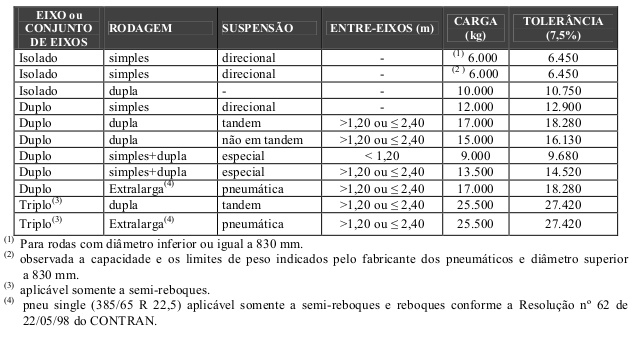
\includegraphics[scale=0.5]{./figuras/tabela-peso-por-eixo.png}
\end{figure}

Os veículos são classificados de acordo com a distribuição dos seus eixos. O \citeonline[p. 15]{tech:dnit-qvf} apresenta uma lista com mais de 150 classificações de veículos, que podem trafegar sem necessidade de AET (Autorização Especial de Trânsito). Quando o fabricante especificar um limite inferior ao da tabela apresentada pelo \citeonline{tech:dnit-qvf}, deve ser considerado o menor valor como referência.

A fiscalização de peso de veículos pesados, em rodovias federias no Brasil, é feita pelos Postos de Pesagem Veicular (PPV) do DNIT e da ANTT, e também pode ser feita através de encaminhamento dos veículos pela Polícia Rodoviária Federal (PRF) a esses postos.

A Figura \ref{fig:ppv} mostra um PPV visto de cima. Nessa imagem é possível identificar uma área maior pavimentada destinada ao patio (B), a sala de controle do PPV (A) e a balança de precisão (C). Na Figura \ref{fig:balanca-precisao} pode ser visto um caminhão passando pela balança de precisão.

\begin{figure}[h!]
  \caption{Posto de Pesagem Veicular (PPV)}
  \label{fig:ppv}
  \centering
    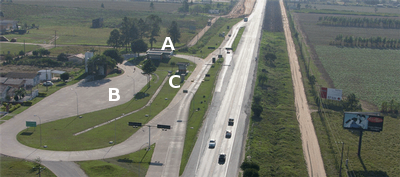
\includegraphics[scale=0.7]{./figuras/ppv_aerea_id.png}
\end{figure}

\begin{figure}[h!]
  \caption{Balança de precisão}
  \label{fig:balanca-precisao}
  \centering
    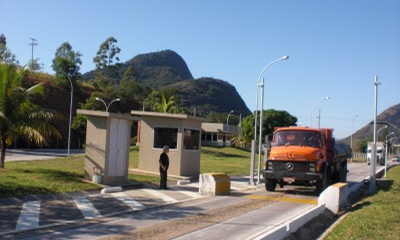
\includegraphics[scale=0.7]{./figuras/balanca-de-precisao.jpg}
\end{figure}

Quando o peso verificado for igual ou inferior ao PBT ou PBTC (peso bruto total combinado) estabelecido para o veículo, acrescido da tolerância de 5\%, porém ocorrer excesso de peso em algum dos eixos, ou conjunto de eixos, acrescido de 5\%, será aplicado a multa sobre a parcela que exceder essa tolerância. Além disso, o veículo somente poderá seguir viagem quando a carga for ser remanejada ou ser feito o seu transbordo, de modo a eliminar os excessos de carga por eixo \cite{tech:dnit-ppv-guia-pratico-operacao}.

\section{Sistemas de pesagem de veículos}\label{sec:ppv-sistemas}
A pesagem de veículos é realizada por sistemas compostos de equipamentos e programas computacionais. Na lista de componentes destes sistemas podem ser encontrados: placas de aquisição, amplificador de carga, sensores, computadores, câmeras de reconhecimento automático de placas de identificação veicular (ALPR), circuitos indutivos, etc. 

Os programas de computador devem ser capazes de processar em tempo hábil informações como: velocidade, distância entre eixos, grupos de eixos, peso por eixo, peso por grupo de eixo, peso bruto total (PBT), classificação do veículo e excesso de peso por eixo e por PBT. Além dessas informações o sistema precisa vinculá-las à identificação do veículo, seja por câmeras ALPR ou seja através de entrada manual dessa informação no sistema.

Além da questão de equipamentos e programas computacionais, é importante salientar a importância das condições estruturais do pavimento para a acurácia dos sistemas de pesagem.

Na Figura \ref{fig:sistema-hswim} é possível visualizar um computador conectado a duas placas de aquisição (equipamentos brancos no centro da imagem) e a um amplificador de carga (equipamento azul no canto superior esquerdo). Essa figura, extraída da revista PÓS-WIM do 1\grad Seminário Internacional de Pesagem em Movimento, é de de um sistema de pesagem em alta velocidade localizada na cidade de Araranguá/SC.

\begin{figure}[h!]
  \caption{Sistema para pesagem em movimento em alta velocidade \cite{magazine:pos-wim-1}}
  \label{fig:sistema-hswim}
  \centering
    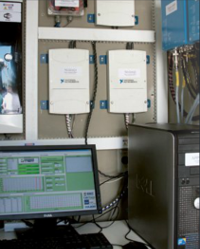
\includegraphics[scale=1]{./figuras/abrigo-pista-experimental.png}
\end{figure}

Nos PPVs sob jurisdição do DNIT, destacam-se duas tecnologias de sensores: \textit{bending plates} e célula de cargas hidráulicas(ou \textit{hydraulic load-cell}).

A tecnologia \textit{bending plate} funciona através de placas metálicas providas de sensores do tipo \textit{strain gages}, localizados na parte de baixo de uma cava especial no pavimento, geralmente com dimensões de 70,0 x 40,0 cm e posicionadas transversalmente ao fluxo de veículos, perfeitamente niveladas com o piso \cite{article:albanorevisando}.

Os sistemas que operam com células de carga hidráulicas (\textit{hydraulic load-cel}), em geral, operam transferindo a carga da roda aplicada sobre a plataforma de pesagem sobre um ou mais cilindros hidráulicos contendo óleo especial, a alteração na pressão hidráulica provocada é correlacionada com a carga por eixo \cite{article:albanorevisando}.

Em \cite[p. 8]{ref:zhang2007evaluating}, é apresentado pelos autores uma tabela comparativa entre os tipos de sensores utilizados na pesagem de veículos. Observa-se que os sensores do tipo \textit{bending plate} são mais baratos que os de células de carga, porém, este último, apresenta acurácia maior dentro de 95\% de confiança (ver Figura \ref{fig:tabela-comparacao-sensores}).

\begin{figure}[h!]
  \caption{Comparação entre sensores de pesagem \cite{ref:zhang2007evaluating}}
  \label{fig:tabela-comparacao-sensores}
  \centering
    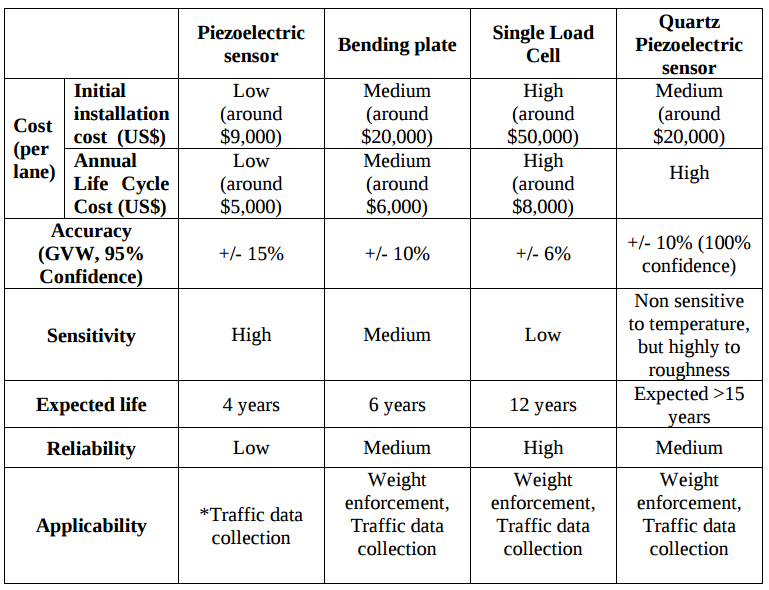
\includegraphics[scale=0.4]{./figuras/tabela-comparacao-siwim.png}
\end{figure}

% ------------------------------------------------------------

\subsection{Algoritmos de apoio à pesagem em movimento}\label{algoritmos}
Um sistema computacional para a pesagem de veículos em movimento consiste essencialmente de:

\begin{itemize}
\item Aquisição de sinal dos sensores de peso (balança);
\item Segmentação sinal (para cortar o respectivo sinal para o caminhão medido);
\item Processamento digital de sinal;
\item Cálculos (velocidade, número de eixos, conjuntos de eixos, distância entre eixos, o peso total, o peso por eixo, peso grupo de eixos, comprimento);
\item Classificação veicular;
\item Calibração;
\item Reconhecimento de placa de identificação veicular;
\item Detecção de infracções;
\end{itemize}

Com base nos resultados da pesagem, classificação e reconhecimento de placa de identificação do veículo, é possível saber se o veículo está com sobrepeso e, em caso afirmativo, é possível vincular a infração à identidade do veículo.

% ------------------------------------------------------------

\chapter{Identificação de padrões para dados e algoritmos}\label{id-standards}

% ------------------------------------------------------------

\chapter{Identificação de padrões tecnológicos compartilhamento de dados e algoritmos}\label{id-tech-standards}

% ------------------------------------------------------------

\chapter{Proposição de padrões para compartilhamento de dados e algoritmos}\label{standards-proposition}

% ------------------------------------------------------------

\chapter{Conclusão}\label{conclusao}

Os efeitos causados por caminhões trafegando acima do limite de carga podem ser sentidos pela deterioração prematuras do pavimento e pelos acidentes ocorridos nas rodovias.

Nesse contexto, é evidente a importância da fiscalização, de modo efetiva, para coibir o tráfego de veículos co sobrepeso.

O sobrepeso e má distribuição da carga poderá prejudicar o condutor em questões de estabilidade, inclinação da iluminação, consumo excessivo de combustível, desgaste desnecessário de peças, custos (multas) e tempo (remanejamento ou transbordo).

Atualmente, no Brasil, os sistemas ainda precisam ser aprimorados para alcançar as condições para a fiscalização e autuação direta. Esse tipo de abordagem permite fiscalizar todos veículos pesados que passarem pela via, de maneira transparente e sem interferir na viagem dos veículos que transitam abaixo dos limites estabelecidos por lei.


\bibliographystyle{ufsc-alf}
\bibliography{bibliografia}

%--------------------------------------------------------
% Elementos pós-textuais

\apendice
\chapter{Teste Apęndice}
\section{Entrevista com o pesquisador Helio Goltsman}

Helio Goltsman é engenheiro pesquisador graduado pela PUC-RJ, especializou-se em planejamento de transportes urbanos pela \textit{Massachusetts Institute of Technology - MIT}. Também foi um dos pioneiros da área de pesagem de veículos pesados no Brasil, atuando desde 1974 nesse tema.

Questionário:

\begin{enumerate}
\item Quais entidades autorizadas a realizar a fiscalização de veículos de carga em rodovias federais?\\
R: Nas rodovias federias, estão autorizados o DNIT e a ANTT. A Polícia Rodoviária Federal (PRF) tem autoridade também de realizar blitz para fiscalizar o peso dos veículos pesados e, se necessário, encaminhá-los ao Posto de Pesagem Veicular (PPV) mais próximo.

\item Quais são os maiores problemas encontrados no passado referentes à pesagem de veículos pesados?\\
R: Havia muito problemas com a pesagem móvel. Esse tipo de pesagem era realizada com uma balança móvel compartilhada com mais de uma localização, tendo que ser transladada diariamente para diferentes localidades. A operação de retirar o equipamento de um posto para instalá-lo em outro, consumia muito tempo, diminuindo o tempo de operação da fiscalização.

\item Quais são os maiores problemas encontrados na atualidade referentes pesagem de veículos pesados?\\
R: Um dos problemas encontrados hoje está relacionado ao alto custo para criar e manter um PPV. Hoje, todos os postos de pesagem federais estão inoperantes por determinação da justiça do trabalho por entender que a operação dos mesmos está terceirizada. 

Outro problema está relacionado com os sistemas de pesagem de pré-seleção. 
Estes sistemas possuem uma margem de erro muito alta, acarretando no encaminhamento de muitos veículos sem sobrepeso para o sistema de pesagem de precisão (baixa velocidade). De acordo com as análises dos dados coletados das pesagens nos postos de pesagem, dos 80\% dos veículos encaminhados à balança de precisão, somente 10\% estão realmente com sobrepeso.

\item Quais são as perspectivas de futuro para a pesagem de veículos pesados?\\
R: O objetivo final é a fiscalização e autuação na velocidade diretriz da via, igual é feito para o controle de velocidade, sem ter o posto de pesagem. Para atender este objetivo, muitas pesquisas ainda deverão ser realizadas ao longo de algumas décadas. Essa questão envolve replanejamento em relação a legislação vigente, ao modo como é feita a pesagem, devem ser estudados tópicos como, por exemplo, a localização das áreas de descarga e descanso. O próximo passo para alcançar esses objetivos será a implantação dos Postos Integrados Automatizados de Fiscalização (PIAFs), onde a pré-seleção na rodovia será feita na velocidade normal da via e, somente quando for constatada a infração, o veículo será encaminhado à balança de precisão do PPV.

\end{enumerate}

\anexo
\chapter{Teste Anexo}
conteúdo do anexo

\end{document}
%%%%%%%%%%%%%%%%%%%%%%%%%%%%%%%%%%%%%%%%%%%%%%%%%%%%%%%%%%%%%%%%%%%%%%%
% Fim do documento                                
%%%%%%%%%%%%%%%%%%%%%%%%%%%%%%%%%%%%%%%%%%%%%%%%%%%%%%%%%%%%%%%%%%%%%%%



%%%%%%%%%%%%%%%%%%%%%%%%%%%%%%%%%%%%%%%%%%%%%%%%%%%%%%%%%%%%%%%%%%%%%%%
% Identificadores do trabalho
% Usados para preencher os elementos pré-textuais
%%%%%%%%%%%%%%%%%%%%%%%%%%%%%%%%%%%%%%%%%%%%%%%%%%%%%%%%%%%%%%%%%%%%%%%

%----------------------------------------------------------------------
% Só preencher se năo for a UFSC - Se for uma instituiçăo "masculina",
% como um Instituto Federal, usar o parâmetro opcional [] - v. exemplo
%
%\instituicao[o]{Instituto Federal do Rio Grande do Sul}

%----------------------------------------------------------------------
% Só preencher se năo for o departamento de Eng. Mecânica - o que deve 
% ser quase que certo. Se for um departamento "feminino", usar o
% parâmetro opcional [] - v. exemplo
%
%\departamento[a]{Faculdade de Cięncias do Mar}

%----------------------------------------------------------------------
% Só preencher se năo for o POSMEC - o que deve ser quase que certo.
% Se for um curso "feminino", usar o parâmetro opcional [] - v. exemplo
%
%\curso[a]{Atividade de Extensăo em Corte e Costura}

%----------------------------------------------------------------------
% Só preencher se năo for tese
% Se for um documento diferente de tese, dissertaçăo, tcc, monografia
% ou relatório, indicar no parâmetro opcional o gęnero - v. exemplo
%
%\documento[o]{Laudo}

%----------------------------------------------------------------------
% Título é obrigatório, mas subtítulo é opcional
%
%\titulo{Elaboraçăo de documentos para a BU/UFSC}
%\subtitulo{Estilo \LaTeX~ Padrăo}

%----------------------------------------------------------------------
% Autor é obrigatório. Năo se atreva a năo incluir ou vai ter surpresa
%
%\autor{Roberto Simoni, Carlos R Rocha}

%----------------------------------------------------------------------
%
% Só preencher se năo for Doutor em Engenharia Mecânica
%\grau{Descomentar se năo for Doutor em Engenharia Mecânica}

%----------------------------------------------------------------------
% Só preencher se năo for Florianópolis
%
%\local{Simcity}

%----------------------------------------------------------------------
% Data deve ter as tręs partes entre chaves
%
%\data{01}{julho}{2010}

%----------------------------------------------------------------------
% Orientador é obrigatório. Coorientador é opcional
% Se o título for diferente (orientadora), indicar como no exemplo
%
%\orientador[Orientadora]{Profa. Dra. Fulana}
%\coorientador{Prof. Dr. Beltrano}

%----------------------------------------------------------------------
% Coordenador do programa é obrigatório
% Se o título for diferente (coordenadora), indicar como no exemplo
%
%\coordenador[Coordenadora]{Profa. Senhora, Dra. Eng.}

%----------------------------------------------------------------------
% Banca - Pode ter até 7 membros além de orientador e co-orientador
% Se estes săo parte da banca, devem ser adicionados com os comandos
% \orientadornabanca{sim} e \coorientadornabanca{sim}
% do contrário, eles aparecerăo antes da designaçăo da banca
% O MembroA da banca é por definiçăo o seu presidente
% O numero total de membros na defesa decide se a folha de aprovaçăo
% deverá ser duplicada. Se passar de 4, uma folha adicional de assinaturas
% será gerada
%
%\numerodemembrosnabanca{4} % Isso decide se haverá uma folha adicional
%\orientadornabanca{sim} % Se faz parte da banca definir como sim
%\coorientadornabanca{sim} % Se faz parte da banca definir como sim
%\bancaMembroA{Prof. Presidente da banca} %Nome do presidente da banca
%\bancaMembroB{Prof. segundo membro}      % Nome do membro da Banca
%\bancaMembroC{Prof. terceiro membro}     % Nome do membro da Banca
%\bancaMembroD{Prof. quarto membro}       % Nome do membro da Banca
%\bancaMembroE{Prof. quinto membro}       % Nome do membro da Banca
%\bancaMembroF{Prof. sexto membro}        % Nome do membro da Banca
%\bancaMembroG{Prof. sétimo membro}       % Nome do membro da Banca

%----------------------------------------------------------------------
% Firulas opcionais - Dedicatória, Agradecimento e Epígrafe
%
% \dedicatoria{Dedicatória para alguem}
% \agradecimento{Agradecimentos, se for o caso...blabla blablablabla blabla ipsum loren e a sophia também blab ablablabl ablbalbalblab lablablbalb lab la}
% \epigrafe{Um bonito pensamento ou citaçăo, se for o caso}{autor do pensamento}

%----------------------------------------------------------------------
% Resumo e abstract - É só definir como mostra o exemplo abaixo
% 
% \textoResumo {Aqui é redigido o resumo do documento...  blabla blablablabla blabla ipsum loren e a sophia também blab ablablabl ablbalbalblab lablablbalb lab lab lab labl a blab lablablab la blab alballbalba lba lba }
% \palavrasChave {chave 1. chave 2. ... chave n.}
% 
% \textAbstract {Here is written the abstract of the document}
% \keywords {key 1. key 2. ... key n.}
